\label{python_functions}
Messwerte werden aus Modbus Registern der unterschiedlichen Komponenten einer \acs{rltanlage} bezogen.  Grundsätzlich wird jeder ausgelesene Wert direkt auf der \acs{rltanzeige} angezeigt, wobei Skalierung und Maßeinheit hinzugefügt werden. In einigen Fällen muss jedoch ein Wert aus mehreren Messwerten abgeleitet werden, eine spezielle Umrechnung oder Ähnliches erfolgen, bevor der Wert auf der \acs{rltanzeige} dargestellt werden kann. In einem solchen Fall wird in der Haupt-Konfigurationsdatei im \enquote{pages} Array (vgl. Kapitel \ref{json_config_files}) der Name einer Python Funktion angegeben, die ausgeführt werden muss, um den erwünschen Wert zu erhalten. 

Diese Python Funktionen sind in der Datei \enquote{modbus\_functions.py} definiert, was den folgenden Vorteil bietet: Ein einfaches Hinzufügen neuer Komponenten, deren Messwerte abgeleitet werden müssen, ohne dass der restliche Code verändert werden muss. Bei der Integration einer neuen Komponente werden lediglich die nötigen Funktionen in der \enquote{modbus\_functions.py} Datei hinzugefügt und diese folgend in der Haupt-Konfigurationsdatei referenziert. Dies ermöglicht eine flexible  Erweiterung des Systems.

Eine solche Python Funktion hat den folgenden grundlegenden Aufbau:
\begin{pythoncode}
def Funktionsname(sensors, additional_info):
	...	
	return Ergebnis
\end{pythoncode}

Jede Funktion erwartet die Übergabeparameter \enquote{sensors} und \enquote{addictional\_info}. \enquote{sensors} ist eine Liste, die Objekte der Klasse \enquote{Sensor} beinhaltet. Ein Objekt der Klasse \enquote{Sensor} wiederum enthält alle erforderlichen Informationen, um einen Wert aus einem Modbus Register auszulesen, wie es in Kapitel \ref{auslesen_rlt_parameter} beschrieben wird. \newline 
Der Parameter \enquote{additional\_info} ermöglicht die Übermittlung weiterer Informationen, falls diese bei der Berechnung oder Ableitung der Werte benötigt werden.

Im folgenden Abschnitt werden die bisher definierten Python Funktionen beschrieben, eine weitere Erklärung zum Ablauf bei der Ausführung der Python Funktionen ist in Kapitel \ref{auslesen_rlt_parameter} zu finden.


\paragraph{Funktion \enquote{standard}}
Diese Funktion wird standardmäßig ausgeführt, wenn in der Haupt-Konfigurationsdatei (vgl. Kapitel \ref{json_config_files}) der Parameter \enquote{python\_function} nicht angegeben wird \bzw keine besondere Python Funktion angegeben wird. Die \enquote{standard} Funktion wird daher als einzige dieser Funktionen nie direkt in der Haupt-Konfigurationsdatei referenziert.

Wie im unten stehenden Code zu sehen ist, wird bei dieser Funktion nichts berechnet. Es wird lediglich die \enquote{get\_data\_from\_modbus} Funktion der \enquote{Sensor} Instanz aufgerufen, welche den Messwert aus dem jeweiligen Modbus Register ausliest und zurück gibt (weitere Erklärung in Kapitel \ref{auslesen_rlt_parameter}).

\begin{pythoncode}
def standard(sensors, additional_info):
	return sensors[0].get_data_from_modbus()
\end{pythoncode}


\paragraph{Funktion \enquote{calc\_rpm}}
Wird verwendet, um bei ebm-papst Ventilatoren die Soll- \bzw Ist-Drehzahl zu ermitteln. Dabei werden, wie im folgenden Code zu sehen ist, zwei Register ausgelesen. Daraufhin wird das Verhältnis der jeweiligen Drehzahl zur maximalen Drehzahl des Ventilators berechnet, das Ergebnis gerundet und in Prozent zurückgegeben.

\begin{pythoncode}
def calc_rpm(sensors, additional_info):
	max_value = sensors[1].get_data_from_modbus()
	rpm_value = (sensors[0].get_data_from_modbus() / 64000) * max_value
	ratio = rpm_value / max_value * 100.0
	return str(round(ratio, 1)) + " %"
\end{pythoncode}

Die Gleichung \eqref{glg:drehzahl_berechnung} für die Berechnung des Wertes \enquote{rpm\_value} stammt aus dem Datenblatt für ebm-papst Ventilatoren \cite[vgl.][118,122]{ebmpapst:2020}: 
\begin{equation}
	\text{rpm\_value}\left[\frac{1}{min}\right] = \frac{\text{Datenbytes}}{64000} \cdot \text{max\_value} \left[\frac{1}{min}\right]
	\label{glg:drehzahl_berechnung}
\end{equation} 

Eine Angabe in der Haupt-Konfigurationsdatei sieht wie folgt aus. Dabei ist zu sehen, dass im \enquote{port} Array zuerst die Quelle der Ist- \bzw Soll-Drehzahl (\enquote{RPMreal} \bzw \enquote{RPMtarget})und als zweites die Quelle der maximalen Drehzahl (\enquote{RPMmax}). Es wird keine \enquote{additional\_info} angegeben.

\begin{jsoncode}
"sources": [
	{
		"port": [
			{"EBM1": "RPMreal"},
			{"EBM1": "RPMmax"}
		],
		"description": "Drehzahl Istwert",
		"python_function": "calc_rpm"
	},
	...
]
\end{jsoncode}



\paragraph{Funktion \enquote{calc\_power}}
Wird verwendet, um den Leistungsverbrauch von ebm-papst Ventilatoren zu ermitteln. Dabei werden, wie im folgenden Code zu sehen ist, drei Register ausgelesen und mit diesen der Leistungsverbrauch berechnet. Daraufhin wird das Ergebnis gerundet und mit der Maßeinheit \enquote{$W$} zurückgegeben.

\begin{pythoncode}
def calc_power(sensors, additional_info):
	byte_value = sensors[0].get_data_from_modbus()
	Uz_value = sensors[1].get_data_from_modbus() / 1000 * 20
	Iz_value = sensors[2].get_data_from_modbus() / 1000 * 2
	power = (byte_value / 65536) * Uz_value * Iz_value
	return str(round(power, 1)) + " W"
\end{pythoncode}

Für die Berechnung des aktuellen Leistungsverbrauchs wurden folgende Gleichungen \eqref{glg:calc_power} \eqref{glg:calc_uz} \eqref{glg:calc_iz} aus dem Datenblatt für ebm-papst Ventilatoren abgeleitet \cite[vgl.][95,126]{ebmpapst:2020}: 
\begin{equation}
	\text{Uz\_value} \left[V\right] = \frac{\text{byte\_value} * 20 \left[mV\right]}{1000}
	\label{glg:calc_uz}
\end{equation} 
\begin{equation}
	\text{Iz\_value} \left[A\right] = \frac{\text{byte\_value} * 2 \left[mA\right]}{1000}
	\label{glg:calc_iz}
\end{equation} 

\begin{equation}
	\text{power} \left[W\right] = \frac{\text{byte\_value}}{65536} \cdot \text{Uz\_value}  \left[V\right] \cdot \text{Iz\_value} \left[A\right]
	\label{glg:calc_power}
\end{equation} 

Eine Angabe in der Haupt-Konfigurationsdatei sieht wie folgt aus. Dabei ist zu sehen, dass im \enquote{port} Array zuerst die Quelle \enquote{Power}, als zweites die Quelle \enquote{Uz} und zuletzt die Quelle \enquote{Iz} eines ebm-papst Ventilators angegeben werden. Es wird keine \enquote{additional\_info} angegeben.

\begin{jsoncode}
"sources": [
	{
		"port": [
			{"EBM1": "Power"},
			{"EBM1": "Uz"},
			{"EBM1": "Iz"}
		],
		"description": "Leistung",
		"python_function": "calc_power"
	},
	...
]
\end{jsoncode}



\paragraph{Funktion \enquote{eng\_status}}
Wird verwendet, um bei ebm-papst Ventilatoren den Motorstatus \bzw aktuelle Fehlermeldungen zu ermitteln. Dabei wird, wie im folgenden Code zu sehen ist, ein Register ausgelesen, worin ein Statuscode enthalten ist. Daraufhin wird dieser Statuscode in eine binäre Zeichenkette konvertiert und seine einzelnen Bits analysiert. Falls ein Bit den Wert \enquote{1} hat, wird zur Zeichenkette \enquote{error\_string} der Fehlercode angehängt. Die Zeichenkette \enquote{error\_string} wird zuletzt zurückgegeben und kann mithilfe des Datenblatt für ebm-papst Ventilatoren \cite[vgl.][119]{ebmpapst:2020} entziffert werden. 

\begin{pythoncode}
def eng_status(sensors, additional_info):
	status = sensors[0].get_data_from_modbus()
	binary_status = bin(status)
	error_string = ""
	counter = 0
	for s in reversed(binary_status):
		counter += 1
		if s == "1":
			if counter == 1:
				error_string += "PHA "
			...
			elif counter == 13:
				error_string += "UzLow "
			else:
				error_string += "Unbekannter Fehler"
			
	if error_string == "":
		error_string = "Kein Fehler"
	
	return error_string
\end{pythoncode}

Eine Angabe in der Haupt-Konfigurationsdatei sieht wie folgt aus. Dabei ist zu sehen, dass im \enquote{port} Array nur die Quelle \enquote{EngStatus} angegeben wird. Es wird keine \enquote{additional\_info} angegeben.

\begin{jsoncode}
"sources": [
	{
		"port": [
			{"EBM1": "EngStatus"}
		],
		"description": "Motorstatus",
		"python_function": "eng_status"
	},
	...
]
\end{jsoncode}



\paragraph{Funktion \enquote{calc\_wrg}}
Wird verwendet, um die Rückwärmzahl einer \acs{rltanlage} zu ermitteln. Diese Zahl, auf die sich unternehmensintern bei Bösch als Wärmerückgewinnungsgrad bezogen wurde, ist ein Maß für die Effizienz der Wärmerückgewinnung. Sie zeigt an, wie viel Wärme aus der Abluft zurückgewonnen werden kann. Die Berechnung der Rückwärmzahl kann entweder auf die Temperatur der Abluft oder der Fortluft bezogen werden, wobei sich hier, wegen der verfügbaren Sensorik, für letztere entschieden wurde. \cite[vgl.][]{Klingenburg:o.J.}\\
Es folgt die Formel \eqref{glg:wrg_berechnung} zur Berechnung der Rückwärmzahl sowie eine Abbildung (Abb. \ref{fig:waermetauscher_wrg}) zur besseren Interpretation: 
\begin{equation}
	\text{Rückwärmzahl} = \frac{\text{Ablufttemperatur} - \text{Fortlufttemperatur}}{\text{Ablufttemperatur} - \text{Außenlufttemperatur}}
	\label{glg:wrg_berechnung}
\end{equation} 

\begin{figure}[H]
	\centering
	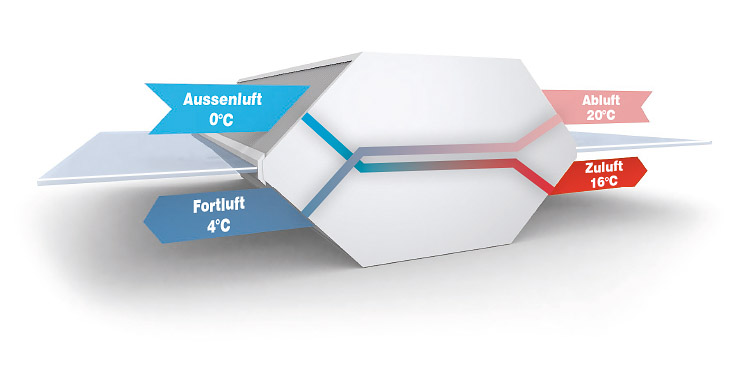
\includegraphics[width=0.7\linewidth]{Bilder/rueckwaermzahl_waermetauscher}
	\caption{Wärmetauscher mit unterschiedlichen Temperaturen (Quelle: \url{http://www.klingenburg.de/fileadmin/user_upload/germany/Wissen/rueckwaermzahlt_de_02.jpg})}
	\label{fig:waermetauscher_wrg}
\end{figure}
 
Die Umsetzung ist im folgenden Code zu sehen. Es werden die drei Temperaturwerte aus den jeweiligen Registern ausgelesen. Daraufhin wird der Wärmerückgewinnungsgrad berechnet, das Ergebnis gerundet und mit der Maßeinheit \enquote{\%} zurückgegeben.

\begin{pythoncode}
def calc_wrg(sensors, additional_info):
	exhaust_air = sensors[0].get_data_from_modbus()  # Abluft
	outgoing_air = sensors[1].get_data_from_modbus()  # Fortluft
	outside_air = sensors[2].get_data_from_modbus()  # Außenluft
	
	wrg = ((exhaust_air - outgoing_air) / (exhaust_air - outside_air)) * 100
	
	return str(round(wrg)) + " %"
\end{pythoncode}

Eine Angabe in der Haupt-Konfigurationsdatei sieht wie folgt aus. Dabei ist zu beachten, dass im \enquote{port} Array zuerst die Quelle der Ablufttemperatur, als zweites die Quelle der Fortlufttemperatur und zuletzt die Quelle der Außenlufttemperatur einer \acs{rltanlage} angegeben werden. Es wird keine \enquote{additional\_info} angegeben.

\begin{jsoncode}
	"sources": [
	{
		"port": [
			{"QBM2": "AI1"},
			{"QBM1": "AI2"},
			{"QBM1": "AI1"}
		],
		"description": "Wärmerückgewinnungsgrad",
		"python_function": "calc_wrg"
	},
	...
	]
\end{jsoncode}



\paragraph{Funktion \enquote{calc\_volume}}
Wird verwendet, um bei ebm-papst Ventilatoren den Volumenstrom zu ermitteln. Dieser gibt an, wie viel Luftvolumen der Ventilator pro Stunde befördert. Zur Bestimmung des Volumenstroms ($q_{V}$) kommt bei ebm-papst das Wirkdruckverfahren zum Einsatz, welches den statischen Druck vor und in der Einströmdüse vergleicht ($\rightarrow$ Differenzdruck der statischen Drücke $\Delta p$).

Die Formel für die Berechnung des Volumenstroms \eqref{glg:volumenstrom_berechnung} ist folgend zu sehen, wobei der K-Faktor \bzw Durchflussfaktor \cite[vgl.][]{rox_klimatechnik:o.J.} von der Größe der Einströmdüse abhängt und aus Datenblättern entnommen wird. \cite[vgl.][171]{ebmpapst:2021}

\begin{equation}
	q_{V}\left[\frac{m^{3}}{h}\right] = \text{K-Faktor} \cdot \sqrt{\Delta p} \left[Pa\right]
	\label{glg:volumenstrom_berechnung}
\end{equation} 

Im unten stehenden Code ist die Anwendung der obigen Formel zu sehen. Der Differenzdruck wird dabei aus einem Modbus Register ausgelesen. In manchen Fällen kann es dazu kommen, dass ein Ventilator nicht dreht. Trotzdem ermittelt der Luftdrucksensor eine kleine Druckdifferenz, welche zu unrealistischen Ergebnissen führt. Daher wird unter einer bestimmten Druckdifferenz ein Volumenstrom von 0 zurückgegeben.

\begin{pythoncode}
def calc_volume(sensors, additional_info):
	sensor_value = sensors[0].get_data_from_modbus()
	
	if sensor_value <= 5:
		return_str = "0 m³/h"
	else:
		return_str = str(round(math.sqrt(sensor_value) * additional_info["k-faktor"])) + " m³/h"
	
	return return_str
\end{pythoncode}

Eine Angabe in der Haupt-Konfigurationsdatei sieht wie folgt aus. Dabei ist zu sehen, dass im \enquote{port} Array die Quelle eines Luftdrucksensors angegeben wird. Der K-Faktor wird als \enquote{additional\_info} angeführt.

\begin{jsoncode}
"sources": [
	{
		"port": [
			{"QBM2": "P1"}
		],
		"description": "ZUL. Volumen",
		"python_function": "calc_volume",
		"additional_info": {"k-faktor": 116}
	},
	...
]
\end{jsoncode}



\paragraph{Funktion \enquote{flap\_position}}
Wird verwendet, um die Klappenposition \bzw den Öffnungsgrad einer Klappe zu ermitteln. 
Dazu wird ein Register ausgelesen, das einen Wert zwischen 0 und 10500 $mV$ enthält \cite[vgl.][17]{siemens:2021}, wie im folgenden Code ersichtlich ist. Anschließend wird das Verhältnis des ausgelesenen Werts zum maximalen Wert von 10500 $mV$ berechnet. Das Ergebnis wird gerundet und in Prozent zurückgegeben.

\begin{pythoncode}
def flap_position(sensors, additional_info):
	flap_mv = sensors[0].get_data_from_modbus()
	flap_pos = flap_mv / 10500 * 100
	return str(round(flap_pos)) + " %"
\end{pythoncode}

Eine Angabe in der Haupt-Konfigurationsdatei sieht wie folgt aus. Im \enquote{port} Array wird die Quelle eines Analog Outputs (AO) eines Siemens QBMs angegeben, an das eine Klappe angeschlossen ist. Es wird keine \enquote{additional\_info} angeführt.

\begin{jsoncode}
"sources": [
	{
		"port": [
			{"QBM1": "AO1"}
		],
		"description": "AUL. Klappe",
		"python_function": "flap_position"
	},
	...
]
\end{jsoncode}



\paragraph{Funktion \enquote{relay\_position}}
Wird verwendet, um die Relaisposition \bzw, ob ein Relais offen oder geschlossen ist, zu ermitteln. Dazu wird ein Register ausgelesen, das einen Wert zwischen 0 und 10500 $mV$ enthält \cite[vgl.][17]{siemens:2021}, wie im folgenden Code ersichtlich ist. Anschließend wird überprüft, ob der ausgelesene Werts größer oder kleiner als die angegebene Schaltschwelle ist. Daraus wird der Zustand des Relais abgeleitet.

\begin{pythoncode}
def relay_position(sensors, additional_info):
	relay_mv = sensors[0].get_data_from_modbus()
	if relay_mv < (additional_info["switching_voltage"] * 1000):
		return "Geschlossen"
	else:
		return "Offen"

\end{pythoncode}

Eine Angabe in der Haupt-Konfigurationsdatei sieht wie folgt aus. Im \enquote{port} Array wird die Quelle eines Analog Outputs (AO) eines Siemens QBMs spezifiziert, an das ein Relais angeschlossen ist. Die Schaltschwelle, also die Spannung, bei der das Relais umschaltet, wird als \enquote{additional\_info} in Volt angegeben.

\begin{jsoncode}
"sources": [
	{
		"port": [
			{"QBM1": "AO2"}
		],
		"description": "WRG. Relais",
		"python_function": "relay_position",
		"additional_info": {"switching_voltage": 8}
	},
	...
]
\end{jsoncode}